\begin{center}\rule{0.5\linewidth}{0.5pt}\end{center}

``To be built to love is to be built to dissolve. It is to be built to unbecome. It is to have the sole purpose in life of falling apart all in the name of someone else.

``We all have a bit of that in us, do we not? You find yourself at a bar or maybe in some class somewhere, you look over, and there they are, right? You look over and you maybe catch their eye and you come undone at the seams. You fall into those big, beautiful eyes — for when you are built to love, every eye that catches yours is the most beautiful thing of all time — and you begin to flake away at the edges.

``And to be built to love is to be all edges. They catch on your clothes, they brush against walls and furniture. You are all edges so that love can fill the cracks and soften those jagged corners.

``You are spiked and barbed. It is as if you are built that way on purpose, so that the slightest breeze can blow you about and catch you up on some future love.''

\AddToHookNext{shipout/after}{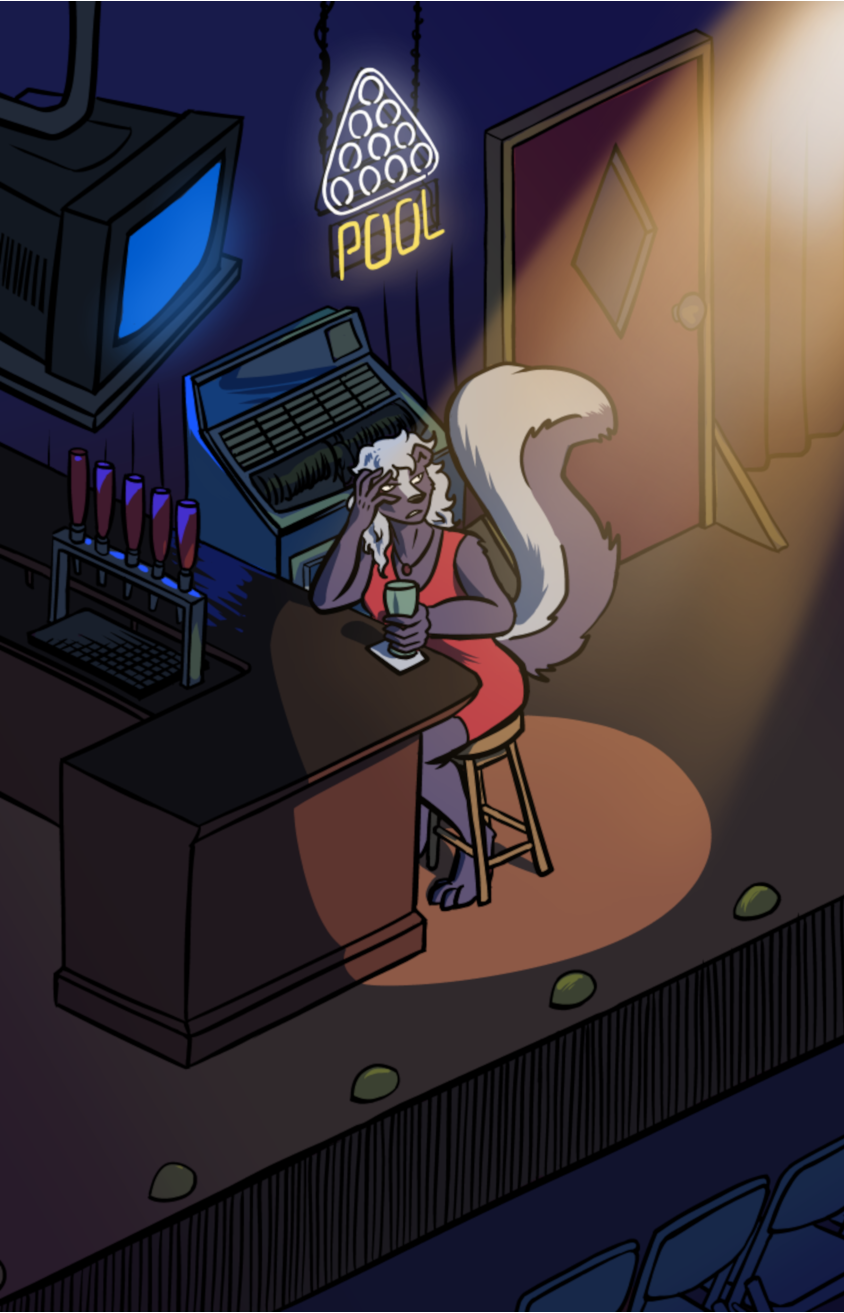
\includepdf[pages={1}]{assets/may-bar}}

The skunk had been sitting on a barstool, hunched over a pint and slurring half to the glass, half to some absent bartender. She slid to her feet, wobbled for a moment, then righted herself.

``Actually, you know what? I have heard it said so many times that to hate — truly hate, burn up inside with that passion — is to actually be in love with the object of your hatred, but I think there is a little bit of hatred in love, too. You fall so completely for someone that you just cannot help but resent them. It is a mirror of that hatred for yourself, for all your jagged edges and prickly burrs, a reflection of the resentment that you feel towards yourself for having been built to love. And look at me!'' She gestured down at herself, a grand sweep of the paw outsized in her intoxication. ``I fuckin' loathe myself! Can you imagine how deeply I must love others, then?''

After a moment's wild laughter, she stumbled back until her tail crumpled against the edge of the stool. ``Ow! Fuck. Yeah, I deserved that one, I think.''

She moved to finish her pint, frowned on finding it empty, and shuffled away from the bar.

``So yeah, you hate yourself, and it actually feels kind of good, does it not? Hatred can fill in those cracks as easily as love. Sure, it may not leave so pretty a pattern as the\ldots whatsit\ldots the patina that stains a tea cup with crackled glaze, but maybe the edges of you do not catch on so many things anymore. Maybe those prickles are dulled and you bounce off everyone around you. You can ping-pong through life, then, loving everyone and loathing yourself.''

The skunk stood up straight again, brushed her shirt out, and brought her tail around to rub at where she'd bumped it against the stool.

``Good Lord, May,'' Ioan said, laughing.

She grinned widely, all that feigned drunkenness suddenly gone from her expression. ``How was it, my dear?''

Ey slouched back against the front row seat ey'd claimed, tapping the end of eir pen against eir lower lip. ``Really, really good,'' ey said. ``Was the stumble intentional?''

``The movement itself was,'' she said. ``Though hitting my tail was not.''

``So no `I deserved that one'?''

She sat down on the edge of the stage, kicking her feet idly. ``It was not in there, no, but I think I will keep it.''

Ey grinned and closed eir notebook around eir pen, setting it aside to stand. ``Yeah, it's good in there,'' ey said, leaning forward to give the bridge of her snout a kiss. She squinted her eyes shut and then scrubbed a paw over her muzzle. ``I mean, the whole thing's good. Only note I really had is that you say `hate' four times in a pretty short span right after you stood up. `That to hate', then `truly hate', then `object of your hatred', and then `little bit of hatred'.''

``Should I make them all different?''

``I'd keep the first two because it works as an echo, so maybe just change the fourth? `Loathing'?''

``Excellent, O great wordsmith.''

Ey laughed and tweaked her ear before hoisting emself up onto the edge of the stage next to her. Predictably, she scooted closer so that she could lean against eir side. ``Who would've thought, hmm? You getting me into theatre and me getting you into writing.''

``This is still theatre! Just earlier on in the process,'' she said, indignant. ``But yes, it is proof that the Bălans can shove us around instead of only the other way around.''

Ey gave her a playful shove with eir shoulder, at which she let out an outsized yelp followed by a whimper. ``So mean!''

``Yeah, that's me. Meanest person you know.''

She rolled her eyes.

Ey let a long silence play then, looking out into the cool darkness of the theater while May summoned up her notebook and scribbled down eir tip from earlier.

``Do you really feel that way?''

``Mm?''

``The jagged edges and self-loathing.''

She shrugged. ``There is some of me in there, yes, but it is still theatre. It is about taking the particular and making it universal, if only for a little while, yes?''

Ey nodded.

When ey didn't reply otherwise, she shrugged and continued, ``I would not say that I agree with that `I loathe myself, so imagine how much I love others' bit. I do not loathe myself, and yet I still love others. Have loved and will love in the future, even, and I see no change in my rare moments of self-loathing.''

Ey laughed. ``\,`Will love in the future'? You leaving me for some handsome guy you met in a bar, then?''

``A bar? Ugh. I am apparently more of a `hunt nerds in the library' type.'' She poked em in the belly. ``But I love \emph{you}, Ioan, and will continue to do so.''

Rubbing at the spot where she'd poked with her dull claw, ey nodded. ``Love you too, May.''

She beamed happily and settled back in against eir side, head resting on eir shoulder. ``I am glad, my dear. I know we agreed early on that this — us being together, I mean — does not need to be permanent, but that does not change the fact that I will continue loving you. Even if we should split, I will not stop.''

Ey nodded slowly.

``I have no plans for such,'' she added quickly. ``You are stuck with me for a good while yet.''

``What? Oh, no,'' ey said, shaking eir head to clear a few too many thoughts. ``I trust you on that. Just got me thinking. Do you still love all the others you've been with?''

She laughed. ``What I said does not apply just to you. Of course I still love them. Some long-diverged forks of me are even still in relationships with their partners.''

``So you've said. You still love them as the root instance, though?''

She nodded. ``I do not begin relationships as anything other than my root instance. I do not know why, but it does not feel fair of me to do anything but.''

``Oh, so none of your forks went on to fork for other relationships?''

``Not that I know of, no. It is a firm conviction, so I would imagine that they hold to it, but perhaps some older ones have diverged. We do not speak much.''

``How many are there, anyway?''

She lifted her head to dot her nose against eir cheek. ``Are you jealous, my dear?'' Her voice was calm and curious. Calm enough and curious enough, some distant part of em noted, that it kept em from falling immediately into defensiveness.

``I get the occasional pangs, more so early on,'' ey said after a long moment's thought. ``When ey was first getting settled in eir relationship, Codrin told me about something that Dear had told em shortly after ey'd been forked, `jealousy is a sign of needs not met'. Whenever I start feeling jealous, that's usually a sign for me to take a step back and think about what need that might be.''

``See, this is what I like about you, Ioan. You feel a thing and then think about it until you understand it. Sometimes a little too much, but it has served you well.''

Ey tilted eir cheek to rest it atop her head, a bit of closeness that also served the purpose of stopping her ear-tip from tickling eir neck.

``I feel a thing and am helpless before it. I cannot but wrap myself up in\ldots it\ldots{}'' she said, pulling out her notebook again to jot down the words as they came. ``Love, hatred, hunger, exhaustion. I am built for them all, and I cannot do a thing about them\ldots{}''

Ey shared a secret smile with emself as the skunk trailed off, continuing to write, tongue-tip peeking out from her muzzle.

``Also,'' she said once she'd finished. ``The answer is that I do not know how many of me are still in relationships. There are at least three, and I know of at least five that have quit, though I declined the merges out of privacy. I never made it a requirement that they keep in touch. Beyond that, I think there are\ldots mm, seven, perhaps?''

``So that makes me your sixteenth relationship?''

``Something like that, yes. Sixteenth truly serious one.'' She slid over and swung her legs up onto the stage so that she could rest her head in eir lap. ``Did my monologue really get you thinking about all this?''

``It's a good monologue,'' ey said, petting over her ears. ``Or start, at least. You said it should be five minutes, right?''

She nodded. ``Around that, yes. I am still working on it.''

``Mmhm. It's good so far, though. It got me thinking, but I'm also just fascinated by you, which helps.''

``Why, because I am weird? I think that is an Odist thing,'' she said, laughing.

``What, am I not allowed to be fascinated by my partner?''

``Absolutely not, no.''

Ey tugged on her ear. ``Fascinated and annoyed.''

``Yes, well, too bad. You remain stuck with me, Mx. Bălan.'' She continued more seriously, ``I did not expect this to be fascinating to you. I try to be careful talking about my other relationships.''

``I don't really mind,'' ey said after giving it due thought. ``That was past May, right? It'd be like getting upset over someone else having exes. If it were multiple partners at the same time, that'd probably be a separate conversation.''

She shook her head. ``I could not do that. I am not built the same as Dear. I am only in multiple relationships in the sense that there are multiple mes, but there is only ever one me involved with one other. It is parallel monogamy.''

``Why?''

``Because,'' she said, rolling onto her back so that she could smile up to em. ``I am also helpless before devotion, and that takes the whole of me.''

``What about Douglas or A Finger Pointing?''

``I hold no romantic feelings for A Finger Pointing.'' She laughed. ``She is nice, but in a boss-you-drink-with-on-Fridays-and-I-guess-occasionally-have-a-fling-with sort of way.''

``And Douglas?''

Her answer was a while in coming. ``Were our friendship to head in that direction, I would fork, but I do not foresee that being the case.''

``Really?'' Ey frowned. ``Wouldn't that be awkward? Us going over there to see him and the other you together?''

``Oh, incredibly awkward,'' she said, rolling her eyes. ``I have done similar in the past, and it would take a year or two to shake out. It is uncomfortable for me, as well, as I am left with the same desire even as my down-tree instance gets fulfillment and they are left with love for you.''

``I can imagine.''

``No, Ioan, I do not think you can,'' she said primly. ``You actually think about the way you feel as you are feeling it like a normal person rather than just crashing headlong into overwhelming emotions like a fucking Odist.''

``Well, fair.''

``I do not think we need to worry about that, though. I am comfortable with my friendship with him just as I am comfortable loving you, and should someone catch my eye--''

``You'd need to start going to more libraries, I think.''

She laughed and shook her head, continuing, ``--should someone catch my eye — or yours, for that matter — we will tackle it then with plenty of talking.''

``Oh, I believe you on that. Skunks never shut up.''

She made as if to bite em on the belly and, when ey flinched away, grinned up to em. ``Mx. Ioan Bălan, you are the one asking all the questions with long, involved answers. Do not pin this on me.''

``Yeah, yeah. You just got me thinking is all. I think you're giving me too much credit saying someone might catch my eye, though.''

``Why?''

Ey shrugged. ``I'm not exactly that observant.''

``You worked as a professional observer for, what, a century?''

``Not \emph{that} kind of observation.''

She laughed. ``Well, okay, yes. I will not discount the possibility, though. If we are in this life for yet more centuries, there is no harm in being deliberate. Plus, I will get an inordinate amount of satisfaction out of seeing you fall for someone. It was so wholesome the first time! I see no reason why it should not be the same subsequent times.''

``I guess. I don't know if there's anyone who--''

She waved a paw dismissively. ``If there is not, there is not. We can speak in hypotheticals like fucking grown-ups.''

``Fine, fine.''

When the silence drew out, May grabbed one of eir hands and started mouthing on eir fingers, sharp skunk teeth just pricking skin.

``Ow!'' Ey laughed and tapped a finger on her nose lightly. ``Pest.''

She licked at eir fingertip, saying, ``Thank you, my dear, in all earnestness. It makes me happy to be able to have a conversation about this.''

``Of course, May. I figure it ought to be an open topic for us.''

She nodded and stretched out on the stage. ``Agreed. We can come back to it later, though. I would like to run this through once more,'' she said, waggling the notebook at em. ``And then head home to get ready for dinner. Debarre is coming over and I plan on flirting with him outrageously in front of you all night long to see if I can make you jealous.''

Ey laughed and pushed at her until she sat up before sliding off the stage and walking back to eir seat. ``Alright. Once more, from the top.''
